\documentclass{article}
\title{The test12 data}
\usepackage{graphicx}
\usepackage{Statweave}
\begin{document}
\maketitle
The data:
\begin{verbatim}
 2  9
16 40
 8 17
18 43
10 25
 4 10
10 27
12 30

\end{verbatim}
The SAS code and output:
\begin{Winput}

options linesize=70;

data test;
    infile "test12.dat";
    input score1 score2;

proc gplot;
    plot score1*score2;
    
proc princomp out=fred;

proc print;
\end{Winput}
\begin{Woutput}
The PRINCOMP Procedure
Observations           8
Variables              2

           Simple Statistics
                score1            score2
Mean       10.00000000       25.12500000
StD         5.45108115       12.66533514

      Correlation Matrix
            score1      score2
score1      1.0000      0.9891
score2      0.9891      1.0000

            Eigenvalues of the Correlation Matrix
        Eigenvalue    Difference    Proportion    Cumulative
   1    1.98907796    1.97815591        0.9945        0.9945
   2    0.01092204                      0.0055        1.0000

           Eigenvectors
               Prin1         Prin2
score1      0.707107      0.707107
score2      0.707107      -.707107

Obs    score1    score2      Prin1       Prin2
 1        2         9      -1.93801    -0.13749
 2       16        40       1.60878    -0.05216
 3        8        17      -0.71306     0.19418
 4       18        43       2.03571     0.03979
 5       10        25      -0.00698     0.00698
 6        4        10      -1.62274     0.06612
 7       10        27       0.10468    -0.10468
 8       12        30       0.53161    -0.01273
\end{Woutput}
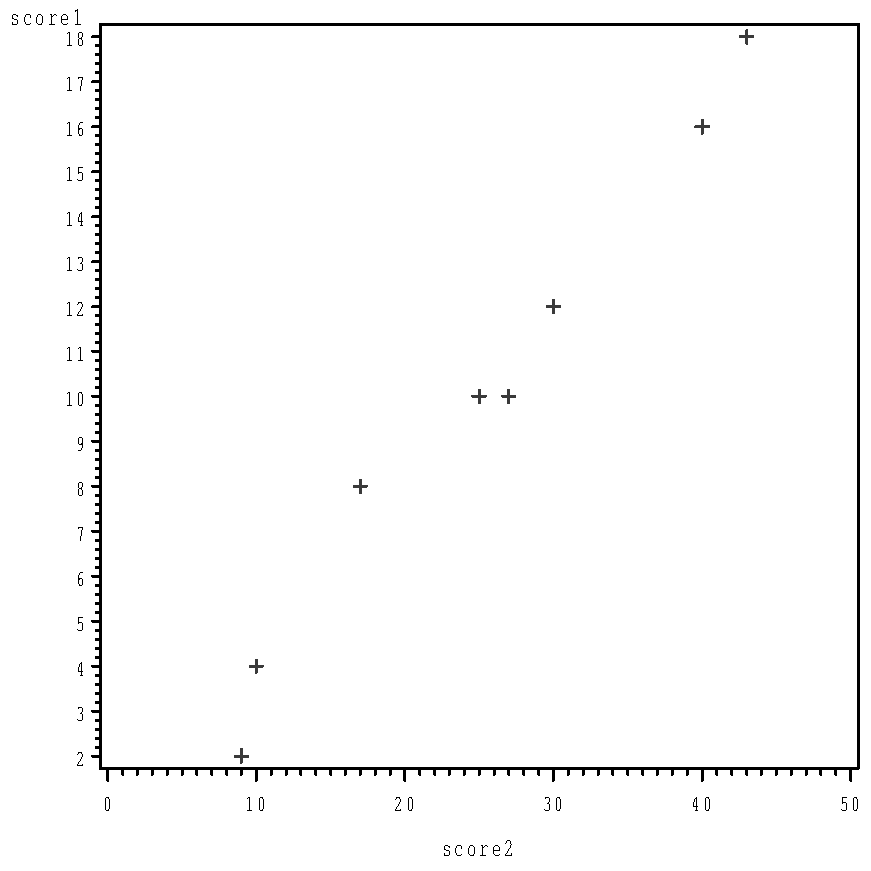
\includegraphics[]{test12-1-SAS-fig.pdf}
\end{document}
